% chapters/ch4_rain.tex --- 第4章 評価結果
\section{評価結果}
\label{sec:evaluation_results}

\subsection{固定間隔の基準特性}
固定間隔における$q_{\mathrm{event}}$($\si{\micro\coulomb}/\text{event}$)と受信品質を基準として整理する.ただし,本節では説明の都合上,電力の従属指標として平均電力の例も併記する.特に,\SI{100}{\milli\second}から\SI{500}{\milli\second}への変更により電力が低下する一方で,受信率や遅延分布が変化するため,制約$\epsilon$に対する可行性が境界条件として現れる.

\subsubsection{固定間隔の平均電力(例)}
本研究では,固定間隔の平均電力を実測し,オフライン評価で用いる電力テーブルとして利用する.表\ref{tab:power_table_example}に,\SI{100}{\milli\second}から\SI{2000}{\milli\second}までの固定間隔における平均電力の一例を示す.

\begin{table}[tb]
  \centering
  \caption{固定間隔の平均電力(例)}
  \label{tab:power_table_example}
  \begin{tabular}{lll}
    \toprule
    広告間隔 [ms] & 平均電力 [mW] & 備考 \\
    \midrule
    100  & 198.56 & n=10(sleep\_on) \\
    500  & 180.80 & n=9(sleep\_on) \\
    1000 & 178.62 & n=9(sleep\_on) \\
    2000 & 177.47 & n=9(sleep\_on) \\
    \bottomrule
  \end{tabular}
\end{table}

\subsubsection{主効果の観察}
表\ref{tab:power_table_example}の例では,\SI{100}{\milli\second}から\SI{500}{\milli\second}への変更で平均電力が大きく低下する.一方で,\SI{500}{\milli\second}以上では改善幅が小さくなる.この傾向は,動的制御において短間隔の滞在時間を抑制する設計が有効であることを示唆する.

\subsection{動的切替(2値制御)の実機確認}
動的制御の最小構成として,\SI{100}{\milli\second}と\SI{500}{\milli\second}の切替を実装し,固定\SI{100}{\milli\second}および固定\SI{500}{\milli\second}と比較する.平均電力が両固定条件の中間に位置し,受信率も中間的になることを確認することで,切替が成立していることを検証する.

切替成立の確認としては,平均電力が両固定条件の中間に位置し,かつログ上でinterval切替が発生することを確認すれば十分である.以降では,TLと$P_{\mathrm{out}}(\tau)$を用いて,QoS制約下での省電力効果を定量評価する.

\subsection{実測のQoS指標(TLとPout)}
本研究では,受信品質をPDRだけでなく,遅延分布と期限超過率$P_{\mathrm{out}}(\tau)$で評価する.特に,非理想スキャン環境では平均受信率が同程度でも,遅延の裾が悪化する場合があるため,$P_{\mathrm{out}}(\tau)$が重要となる(\secref{sec:metrics_detail}).

\subsubsection{実測例(D2b,scan90)}
表\ref{tab:d2_summary}に,D2b(scan90)における実測例を示す.本表は,S1/S4の2条件について,固定\SI{100}{\milli\second},固定\SI{500}{\milli\second},および方策(2値切替)の比較をまとめたものである.ここでは run B(n=3)と追加取得 B/02(n=3)を統合し,各条件n=6として集計した.

\begin{table}[tb]
  \centering
  \caption{D2b(scan90)の実測例(mean$\pm$std, 各n=6)}
  \label{tab:d2_summary}
  {\small
  \setlength{\tabcolsep}{4pt}
  \begin{tabular}{lrrrrr}
    \toprule
    条件 & Pout(1s) & TL\_mean[s] & PDR\_u & P[mW] & share100 \\
    \midrule
    S1-100   & 0.075$\pm$0.027 & 3.76$\pm$1.46 & 0.789$\pm$0.016 & 204.1$\pm$1.4 & 1.000$\pm$0.000 \\
    S1-500   & 0.142$\pm$0.049 & 5.29$\pm$0.02 & 0.816$\pm$0.018 & 184.7$\pm$1.5 & 0.000$\pm$0.000 \\
    S1-policy & 0.125$\pm$0.027 & 5.24$\pm$0.05 & 0.803$\pm$0.022 & 191.5$\pm$1.9 & 0.331$\pm$0.004 \\
    \midrule
    S4-100   & 0.053$\pm$0.010 & 1.25$\pm$0.01 & 0.792$\pm$0.009 & 204.4$\pm$2.1 & 0.998$\pm$0.002 \\
    S4-500   & 0.146$\pm$0.031 & 2.48$\pm$1.11 & 0.817$\pm$0.020 & 184.5$\pm$1.5 & 0.000$\pm$0.000 \\
    S4-policy & 0.069$\pm$0.029 & 1.58$\pm$0.50 & 0.793$\pm$0.021 & 196.6$\pm$1.6 & 0.595$\pm$0.008 \\
    \bottomrule
  \end{tabular}
  }
\end{table}

\begin{figure}[tb]
  \centering
  \includegraphics[width=0.90\linewidth]{../uccs_d2_scan90/plots/d2b_B_n6_power_vs_pout}
  \caption{D2b(run B + B/02, n=6)における平均電力と$P_{\mathrm{out}}(1\mathrm{s})$の関係(share100を注釈)}
  \label{fig:d2b_power_vs_pout}
\end{figure}

\subsubsection{解釈}
表\ref{tab:d2_summary}および図\ref{fig:d2b_power_vs_pout}より,方策(2値切替)はFixed100より低電力であり,Fixed500より低い期限超過率(QoS改善)を示す運用点になり得る.さらに,遷移が多い側(S4)ほどshare100が増加しており,「必要時だけ\SI{100}{\milli\second}に寄せ,それ以外は\SI{500}{\milli\second}に寄せる」挙動が定量で確認できる.

また,平均電力はFixed100/Fixed500の滞在比率(share100)による線形混合で概ね説明できるため,方策の省電力効果はinterval滞在比率に支配されることが示唆される.これにより,「sleep差分が効いた/効かなかった」といった実装依存の議論から切り離し,制御則(どの状態で短間隔へ戻すか)の議論へ接続しやすくなる.

\subsubsection{条件悪化時の頑健性(D3,scan70)}
\label{sec:d3_scan70}
表\ref{tab:d3_summary}に,scan dutyを低下させたD3(scan70, S4, 各n=3)の結果を示す.scan70ではFixed500の期限超過率が0.285まで悪化する一方で,方策は0.089まで改善し,Fixed100(0.065)と同様に制約$\epsilon$(例:$\epsilon=0.1$)を満たす.このとき方策はFixed100より平均電力を\SI{7.8}{\milli\watt}(約3.7\%)低減するが,Fixed500よりは\SI{12.6}{\milli\watt}高い.

なお,scan70では受信欠落によりRXタグ由来の短間隔滞在比率$\hat{\rho}_{100}$(約0.42)が過小評価されやすいため,D3では平均電力の線形混合により$\hat{\rho}_{100}$を推定した.固定\SI{100}{\milli\second}/\SI{500}{\milli\second}の平均電力をそれぞれ$P_{100}, P_{500}$とし,方策の平均電力を$P_{\mathrm{policy}}$とすると,$\hat{\rho}_{100}=(P_{\mathrm{policy}}-P_{500})/(P_{100}-P_{500})$で与えられる.また,SDコピーでmtimeが信頼できないため,TXSDログはadv\_count(tick\_count)でクラスタリングしてRXと対応付けた.

\begin{table}[tb]
  \centering
  \caption{D3(scan70, S4)の実測例(mean$\pm$std, 各n=3)}
  \label{tab:d3_summary}
  {\small
  \setlength{\tabcolsep}{4pt}
  \begin{tabular}{lrrrr}
    \toprule
    条件 & Pout(1s) & TL\_mean[s] & P[mW] & $\hat{\rho}_{100}$ \\
    \midrule
    S4-100   & 0.065$\pm$0.028 & 1.34$\pm$0.02 & 209.9$\pm$0.5 & 1.000 \\
    S4-500   & 0.285$\pm$0.061 & 2.93$\pm$1.07 & 189.5$\pm$0.5 & 0.000 \\
    S4-policy & 0.089$\pm$0.037 & 1.40$\pm$0.07 & 202.1$\pm$0.1 & 0.618 \\
    \bottomrule
  \end{tabular}
  }
\end{table}

\subsubsection{U-shuffleアブレーション(D4,scan90)}
\label{sec:d4_ablation}
D2bの主結果に対して,「不確実度$U$は本当に効いているか(単なる閾値遊びではないか)」という疑問に答えるため,D4としてアブレーション実験を行った.ここでは制御器の構造と閾値は固定し,不確実度系列$U$の時間整合だけを破壊する(shuffleする)ことで,制御がどのように崩れるかを観察する.

表\ref{tab:d4_summary}に,S4(遷移が多い条件)における結果(各n=3)を示す.方策(U+CCS)はFixed100より低電力であり,Fixed500より低い期限超過率を示す運用点になり得る.一方で,$U$をshuffleするとshare100が0.593から0.943へ増加し,adv\_countも1227から1715へ増加してFixed100に近い挙動へ崩れる.その結果,平均電力も200.5\,mWから208.1\,mWへ増加し,省電力効果が失われる(図\ref{fig:role_separation_overview}).

\begin{table}[tb]
  \centering
  \caption{D4(scan90, S4)のアブレーション結果(mean$\pm$std, 各n=3)}
  \label{tab:d4_summary}
  {\small
  \setlength{\tabcolsep}{4pt}
  \begin{tabular}{lrrrrr}
    \toprule
    条件 & Pout(1s) & TL\_mean[s] & P[mW] & adv\_count & share100 \\
    \midrule
    Fixed100 & 0.049$\pm$0.000 & 1.24$\pm$0.01 & 208.2$\pm$1.3 & 1796$\pm$0 & 1.000$\pm$0.000 \\
    Fixed500 & 0.130$\pm$0.014 & 1.59$\pm$0.06 & 187.9$\pm$0.8 & 359$\pm$0 & 0.000$\pm$0.000 \\
    Policy(U+CCS) & 0.098$\pm$0.024 & 1.28$\pm$0.01 & 200.5$\pm$0.8 & 1227$\pm$0 & 0.593$\pm$0.009 \\
    Ablation(U-shuf) & 0.049$\pm$0.000 & 1.23$\pm$0.01 & 208.1$\pm$0.3 & 1715$\pm$0 & 0.943$\pm$0.000 \\
    \bottomrule
  \end{tabular}
  }
\end{table}

\subsubsection{CCS-offアブレーション(D4B,scan90)}
\label{sec:d4b_ccs_off}
CCSの寄与を切り分けるため,制御則の構造は固定したままCCSを無効化し,不確実度$U$のみで切替を行う(U-only)実験(D4B)を追加した.
表\ref{tab:d4b_summary}にS4の結果(各n=3)を示す.Policy(U+CCS)とU-only(CCS-off)は平均電力がほぼ同一(ともに約200.6\,mW)で,adv\_countおよび$\hat{\rho}_{100}$も同等であるにも関わらず,Policy(U+CCS)の方が$P_{\mathrm{out}}(1\mathrm{s})$とTL\_meanが改善する.したがって,CCSは「\SI{100}{\milli\second}を増やす」ことでなく,同じ短間隔予算の範囲で「短間隔を使うタイミング」を調整することでQoSを改善していると解釈できる(図\ref{fig:role_separation_overview}).

\begin{table}[tb]
  \centering
  \caption{D4B(scan90, S4)のCCS-offアブレーション結果(mean$\pm$std, 各n=3)}
  \label{tab:d4b_summary}
  {\small
  \setlength{\tabcolsep}{4pt}
  \begin{tabular}{lrrrrr}
    \toprule
    条件 & Pout(1s) & TL\_mean[s] & P[mW] & adv\_count & $\hat{\rho}_{100}$ \\
    \midrule
    Fixed100 & 0.081$\pm$0.014 & 1.49$\pm$0.11 & 208.3$\pm$0.5 & 1796$\pm$0 & 1.000 \\
    Fixed500 & 0.130$\pm$0.028 & 1.21$\pm$0.26 & 188.1$\pm$0.3 & 359$\pm$0 & 0.000 \\
    U-only(CCS-off) & 0.065$\pm$0.014 & 1.41$\pm$0.15 & 200.6$\pm$0.2 & 1227$\pm$0 & 0.621 \\
    Policy(U+CCS) & 0.049$\pm$0.000 & 1.32$\pm$0.03 & 200.6$\pm$0.1 & 1215$\pm$0 & 0.620 \\
    \bottomrule
  \end{tabular}
  }
\end{table}

\begin{figure}[tb]
  \centering
  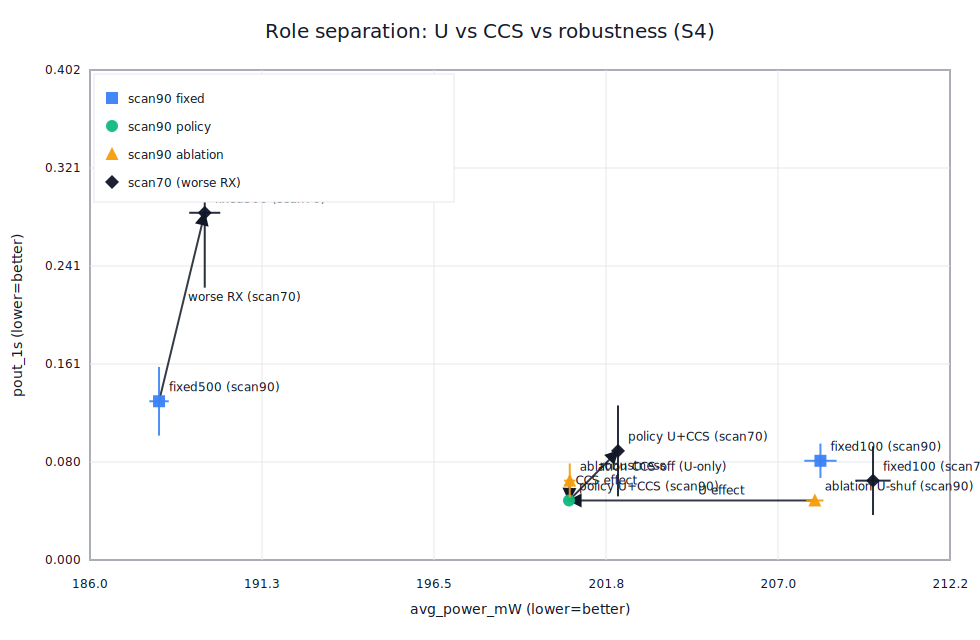
\includegraphics[width=0.95\linewidth]{../uccs_d4b_scan90/plots/role_separation_d3_d4_d4b}
  \caption{U/CCSの役割分離と頑健性のまとめ(S4): 平均電力と$P_{\mathrm{out}}(1\mathrm{s})$の関係(D3/D4/D4B)。図中の矢印は,Uの寄与(U-shuffleから方策へ),CCSの寄与(CCS-offから方策へ),および受信条件悪化(scan90からscan70)に対する挙動を示す.}
  \label{fig:role_separation_overview}
\end{figure}

\subsubsection{補足:CCS-off追試(D4B,scan70)}
\label{sec:d4b_scan70_followup}
受信条件を悪化させたscan70でもCCS-offアブレーション(D4B)の追試を行い,S4(各n=3)で集計した(出力:\texttt{\detokenize{uccs_d4b_scan70/metrics/01_fixed/}}).表\ref{tab:d4b_scan70_summary}に示すように,Fixed500は$P_{\mathrm{out}}(1\mathrm{s})=0.228\pm0.037$まで悪化する一方で,Policy(U+CCS)およびU-only(CCS-off)は0.02以下に改善し,平均電力もFixed100より\SI{4}{\milli\watt}程度低い.したがって,受信条件悪化時でも方策群が中間解として成立し得ることが確認できる.

一方で,本追試ではU-onlyの$\hat{\rho}_{100}$が0.780でPolicy(0.735)よりわずかに大きく,$P_{\mathrm{out}}(1\mathrm{s})$もU-onlyの方が小さい.このため,本条件単体から「同電力でCCSがQoSを改善する」とは言い切れず,同mixでQoS差が出たscan90の結果(表\ref{tab:d4b_summary})を主張の根拠とする.

\begin{table}[tb]
  \centering
  \caption{D4B(scan70, S4)の追試結果(mean$\pm$std, 各n=3)}
  \label{tab:d4b_scan70_summary}
  {\small
  \setlength{\tabcolsep}{4pt}
  \begin{tabular}{lrrrrr}
    \toprule
    条件 & Pout(1s) & TL\_mean[s] & P[mW] & adv\_count & $\hat{\rho}_{100}$ \\
    \midrule
    Fixed100 & 0.024$\pm$0.024 & 0.43$\pm$0.32 & 206.4$\pm$0.5 & 1800$\pm$0 & 1.000 \\
    Fixed500 & 0.228$\pm$0.037 & 1.44$\pm$0.51 & 187.6$\pm$0.4 & 360$\pm$0 & 0.000 \\
    U-only(CCS-off) & 0.008$\pm$0.014 & 0.24$\pm$0.13 & 202.2$\pm$1.2 & 1323$\pm$0 & 0.780 \\
    Policy(U+CCS) & 0.016$\pm$0.014 & 0.30$\pm$0.14 & 201.4$\pm$1.0 & 1323$\pm$0 & 0.735 \\
    \bottomrule
  \end{tabular}
  }
\end{table}

\subsubsection{解釈(D4/D4B)}
D4の結果は,制御器の構造と閾値を固定したまま入力$U$の時間整合だけを破壊すると,制御が短間隔(\SI{100}{\milli\second})に張り付く方向へ崩れることを示している.一方でD4Bの結果は,平均電力(=短間隔滞在量)をほぼ同一に保ったまま,CCSの有効化によって$P_{\mathrm{out}}(1\mathrm{s})$とTL\_meanが改善することを示している.したがって,本研究の2値制御では,$U$が「どれだけ短間隔を使うか(電力)」を決め,CCSが「いつ短間隔を使うか(QoS)」を改善する,という役割分担が示唆される.

\subsubsection{効果量のブートストラップCI(追加検証)}
各条件$n=3$のため,trial単位の差分に対してpercentile bootstrap($n_{\mathrm{boot}}=20000$)で効果量の不確かさを確認した.D4Bでは,$\Delta P_{\mathrm{out}}(1\mathrm{s})$(U+CCS $-$ U-only)$=-0.0163$で95\%CIは$[-0.0244, 0.0000]$となり,$\Delta power$は$-0.0235$\,mWで95\%CIが$[-0.2332, 0.1886]$となった.また,D4では$\Delta power$(policy $-$ U-shuf)$=-7.58$\,mW(95\%CI $[-8.39,-6.93]$),$\Delta P_{\mathrm{out}}(1\mathrm{s})=+0.0488$(95\%CI $[0.0244,0.0732]$)であり,U-shuffleが短間隔寄りに崩れることが定量で確認できる.さらに,D3では$\Delta P_{\mathrm{out}}(1\mathrm{s})$(policy $-$ fixed500)$=-0.195$(95\%CI $[-0.260,-0.130]$),$\Delta power$(policy $-$ fixed100)$=-7.76$\,mW(95\%CI $[-8.24,-7.22]$)であり,受信条件悪化時でも方策がFixed500より低い期限超過率を示しつつFixed100より低電力であることが裏付けられる.

\subsubsection{$\hat{\rho}_{100}$--$P_{\mathrm{out}}$プロット(追加検証)}
滞在比率の推定を直感的に扱うため,固定\SI{100}{\milli\second}/\SI{500}{\milli\second}の平均電力を$P_{100},P_{500}$とし,各条件の平均電力$P$から
\begin{equation}
  \hat{\rho}_{100} = \frac{P-P_{500}}{P_{100}-P_{500}}
\end{equation}
を定義する($\hat{\rho}_{100}\approx share100_{\mathrm{mix}}$).図\ref{fig:rho100_vs_pout_overview}は,$x=\hat{\rho}_{100}$,$y=P_{\mathrm{out}}(1\mathrm{s})$としてD3/D4/D4Bを同一平面に配置したものである.D4Bでは,Policy(U+CCS)とU-only(CCS-off)が同程度の$\hat{\rho}_{100}$であるにも関わらず$P_{\mathrm{out}}$が改善し,同電力でQoSが改善する傾向が可視化できる.また,D4(U-shuffle)では$\hat{\rho}_{100}$が1に近づき,短間隔へ張り付く崩れ方が確認できる.

\begin{figure}[tb]
  \centering
  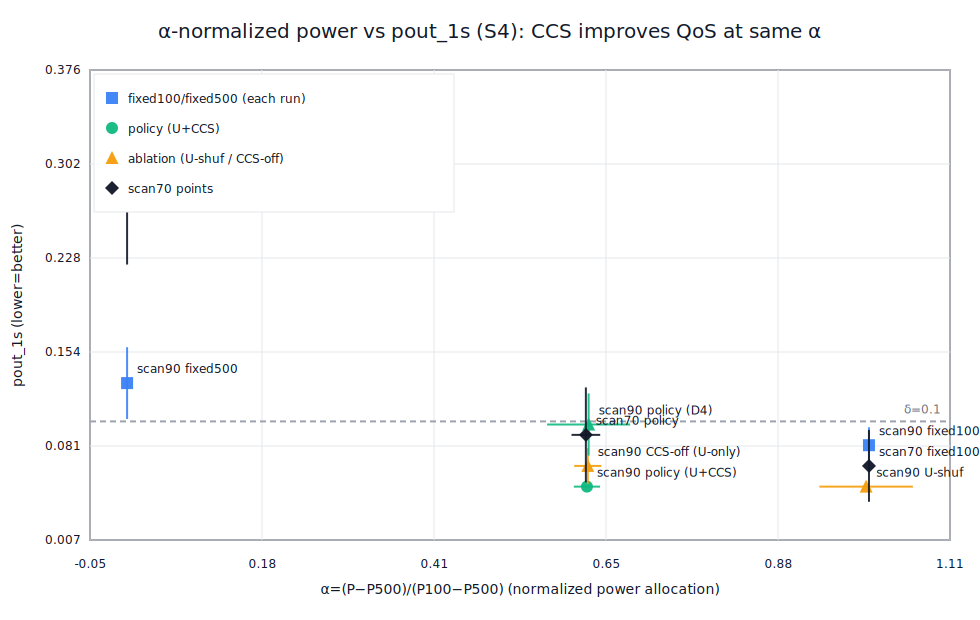
\includegraphics[width=0.95\linewidth]{../uccs_d4b_scan90/plots/alpha_vs_pout_overview}
  \caption{$\hat{\rho}_{100}$(\SI{100}{\milli\second}滞在比率の推定値)と$P_{\mathrm{out}}(1\mathrm{s})$の関係(D3/D4/D4B).図中の$\epsilon=0.1$は制約の例として示す.}
  \label{fig:rho100_vs_pout_overview}
\end{figure}

\subsubsection{事例解析:同電力でQoS差を生んだ少数イベント(D4B run01)}
D4B(run01)では,Policy(U+CCS)とU-only(CCS-off)が同程度の平均電力でありながら$P_{\mathrm{out}}(1\mathrm{s})$が異なる.この差の内訳を確認するため,trial$\times$遷移ごとのTLを集計し,outage(TL$>\SI{1}{\second}$)に寄与した遷移をランキングした(出力:\texttt{\detokenize{uccs_d4b_scan90/plots/outage_story_01/}}).代表例として\texttt{\detokenize{transition_step=1128}}(2$\rightarrow$9)では,U-onlyでTL$\approx\SI{9.889}{\second}$(outage)だがPolicyではTL$\approx\SI{0.212}{\second}$であり,少数の失敗イベントが$P_{\mathrm{out}}$差を生み得ることが確認できる.さらに,遷移単位の集計から復元したoutage率(\texttt{\detokenize{pout_est}})がsummaryと一致することを確認した(Policy=0.04878, U-only=0.06504).

\begin{figure}[tb]
  \centering
  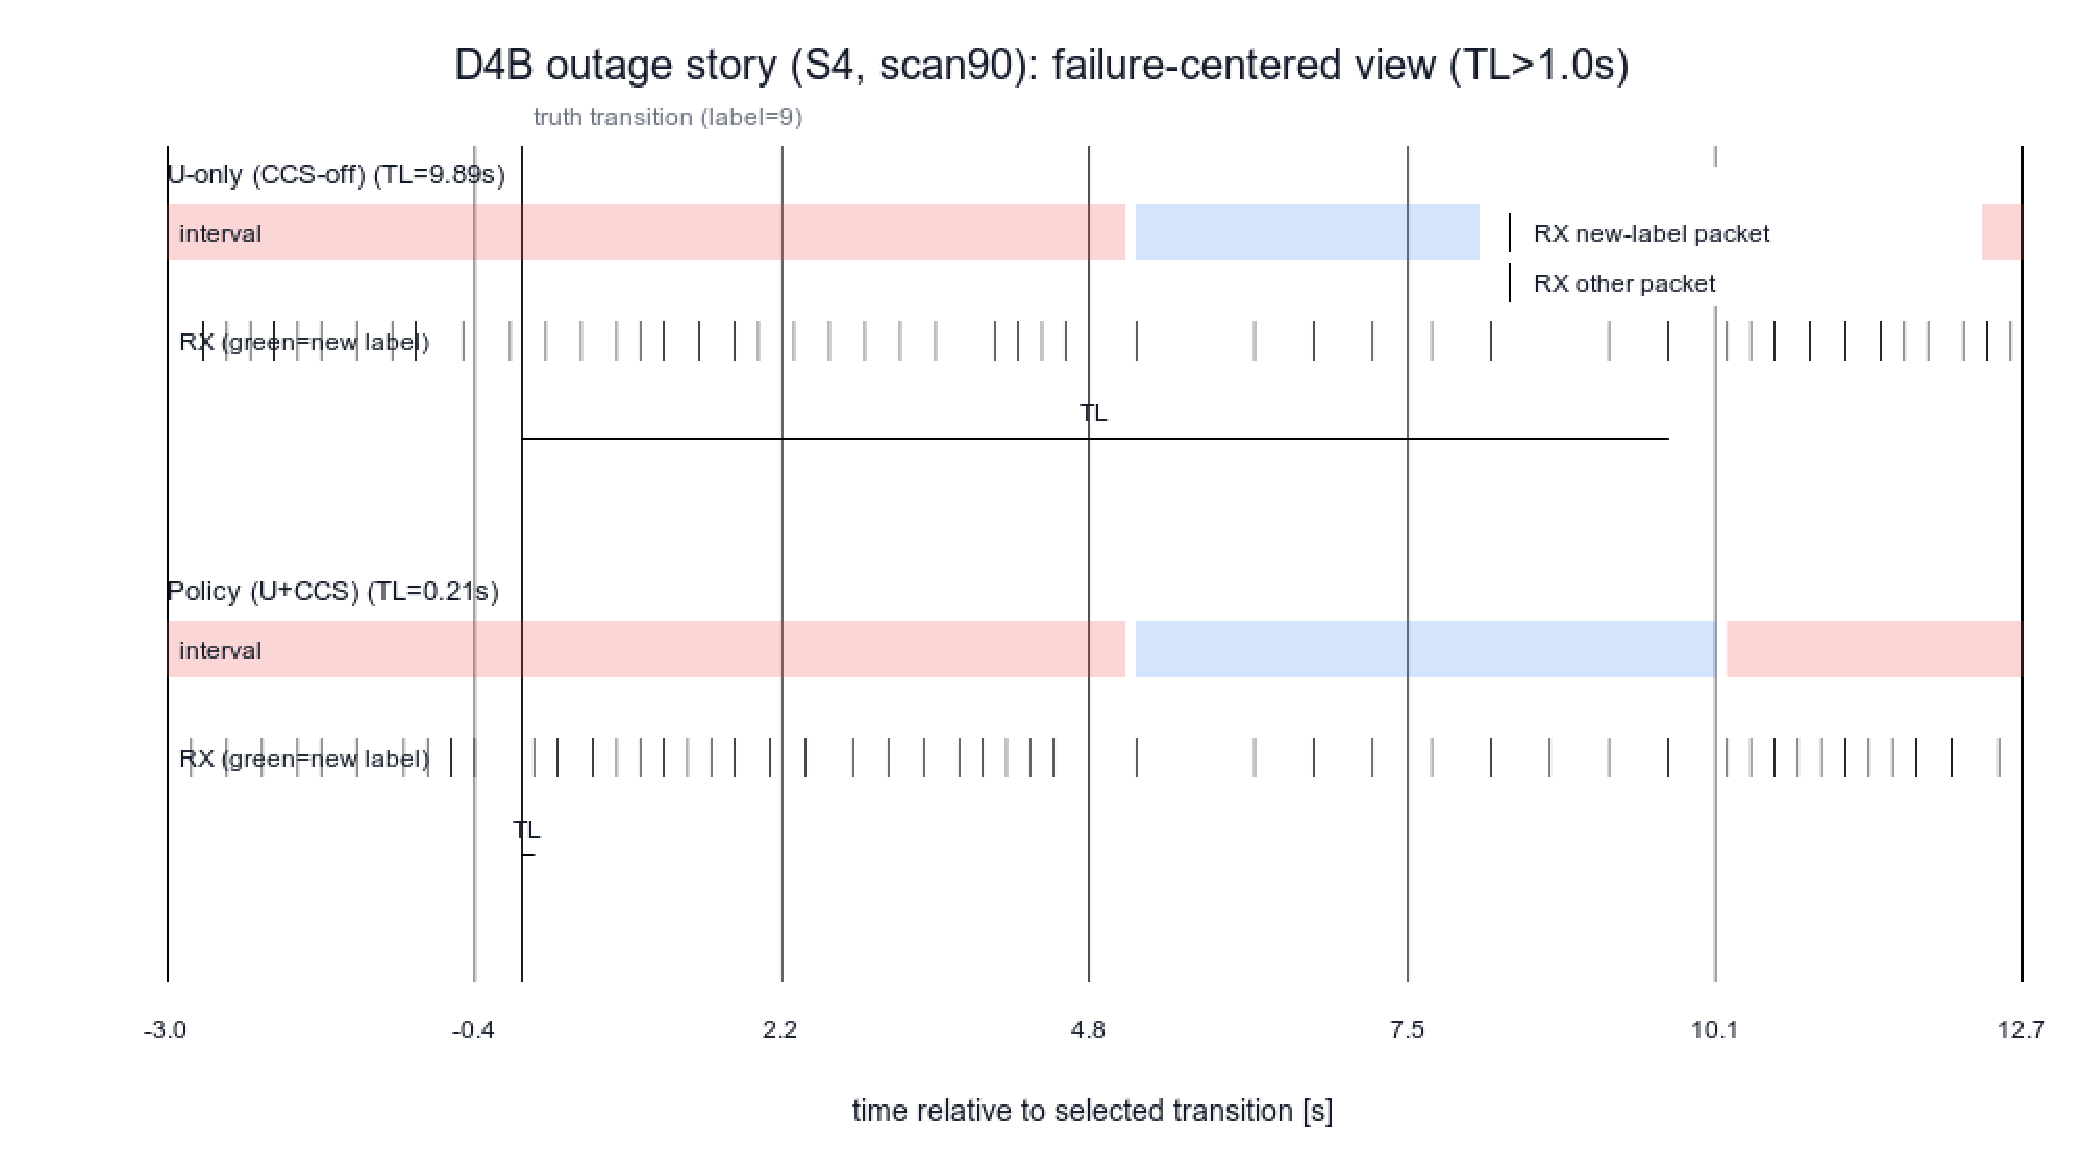
\includegraphics[width=0.98\linewidth]{../uccs_d4b_scan90/plots/outage_story_01/fig_outage_timeline}
  \caption{D4B(run01)における失敗イベント中心のタイムライン図(例:\texttt{\detokenize{transition_step=1128}}, 2$\rightarrow$9).U-onlyではTLが長くoutageとなる一方で,Policy(U+CCS)では短時間で受信されoutageが回避される.}
  \label{fig:outage_story_timeline}
\end{figure}

\subsubsection{尾(TL$>\SI{1}{\second}$)への寄与分解(D4B run01)}
$P_{\mathrm{out}}(1\mathrm{s})$は「TL$>\SI{1}{\second}$となるoutageの発生有無」で決まりやすい.そこで,trialごとのoutage回数分布と,$\Delta P_{\mathrm{out}}$(U-onlyが悪化する差分)が「どの遷移に集中しているか」を可視化した(出力:\texttt{\detokenize{uccs_d4b_scan90/plots/pout_tail_01/}}).図\ref{fig:d4b_pout_tail_decomposition}より,本run01では正の$\Delta P_{\mathrm{out}}$を持つ遷移は41遷移中2遷移であり,上位1遷移で差分の50\%を説明するなど,尾の差が少数遷移へ強く集中していることが確認できる.

\begin{figure}[tb]
  \centering
  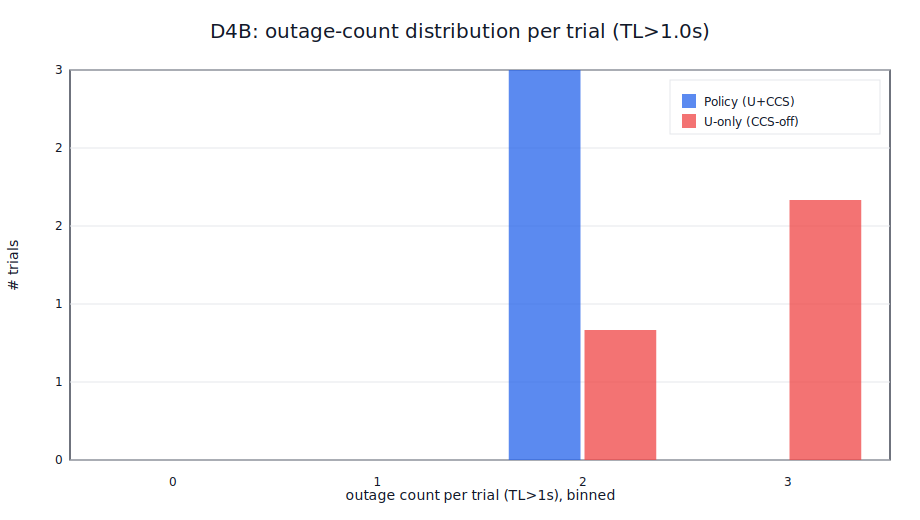
\includegraphics[width=0.92\linewidth]{../uccs_d4b_scan90/plots/pout_tail_01/fig_outage_count_hist}
  \vspace{2mm}
  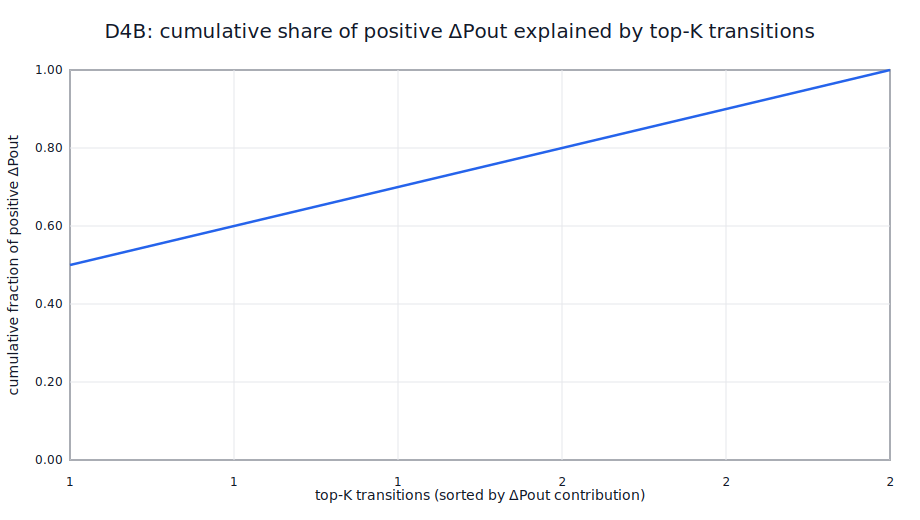
\includegraphics[width=0.92\linewidth]{../uccs_d4b_scan90/plots/pout_tail_01/fig_delta_pout_cum}
  \caption{D4B(run01)における尾(TL$>\SI{1}{\second}$)の寄与分解.(上)trialごとのoutage回数分布,(下)上位K遷移が$\Delta P_{\mathrm{out}}(1\mathrm{s})$をどれだけ説明するか(累積寄与).}
  \label{fig:d4b_pout_tail_decomposition}
\end{figure}

\subsubsection{条件付きタイミング:失敗遷移近傍の短間隔割当て(D4B run01)}
同電力で$P_{\mathrm{out}}$差が生じる要因として,平均的な$\hat{\rho}_{100}$(滞在比率)ではなく「どのタイミングで短間隔を割り当てたか」が効いている可能性がある.そこで,U-onlyのoutage率が高い遷移(差分上位)に限定し,遷移近傍における$P(\text{interval}=\SI{100}{\milli\second})$を再集計した(出力:\texttt{\detokenize{uccs_d4b_scan90/plots/ccs_timing_conditional_01/}}).図\ref{fig:d4b_ccs_timing_conditional}は,失敗しやすい遷移近傍では短間隔割当ての差が現れやすいことを示しており,CCSが「同じ短間隔予算の使い方(タイミング)」を通じてQoSを改善する可能性を支持する.

\begin{figure}[tb]
  \centering
  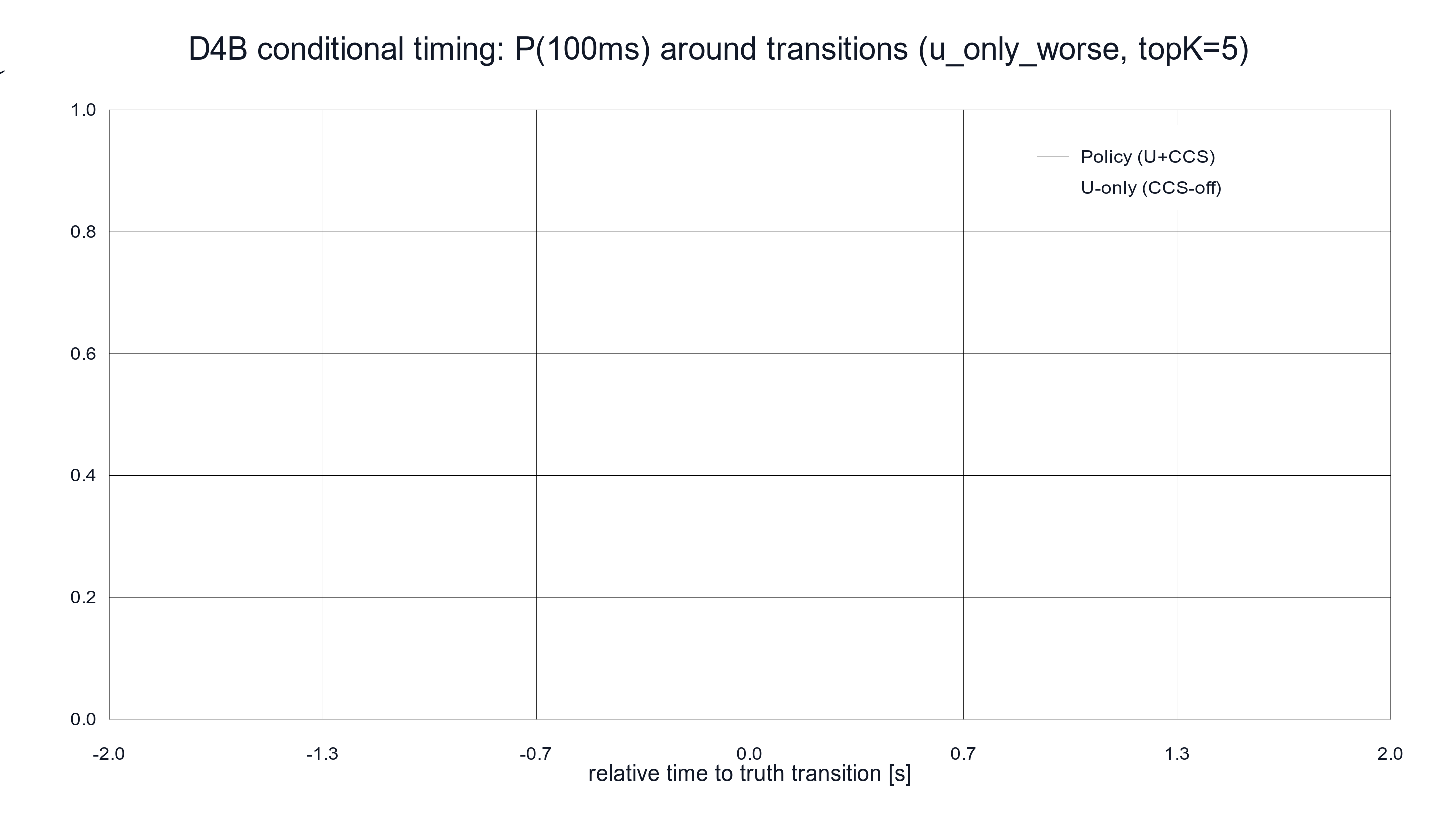
\includegraphics[width=0.95\linewidth]{../uccs_d4b_scan90/plots/ccs_timing_conditional_01/fig_event_triggered_p100_conditional}
  \caption{D4B(run01)における条件付きタイミング分析:U-onlyが悪化する遷移(差分上位)に限定し,遷移近傍の$P(\text{interval}=\SI{100}{\milli\second})$を可視化した.}
  \label{fig:d4b_ccs_timing_conditional}
\end{figure}
\clearpage

\subsection{オフライン評価との整合}
オフライン評価で予測される運用点と,実機で得られる平均電力・受信品質の差分を比較し,推定モデルの妥当性と限界を整理する.

\subsubsection{予測と実測の差分}
オフライン評価は,固定間隔の電力テーブルと受信品質推定を合成するため,実環境の非理想性を完全には表現しない.したがって,予測値は「候補探索と説明のための近似」として用い,実測との差分を評価しながらモデルの限界を記述することが重要である.

\subsubsection{制約帯プロット(参考)}
制約帯プロットは,\secref{sec:offline_eval}の図\ref{fig:letter_delta_band}に示した通り,固定間隔点と候補方策点の位置関係を俯瞰し,実機評価で探索すべき領域を絞り込むための近似として有効である.

\subsection{まとめ}
本節の結果を,次章の考察に接続するために要点を整理する.
\begin{itemize}
  \item D2b(scan90, n=6)では,方策(2値切替)がFixed100より低電力で,Fixed500より低い期限超過率を示す運用点になり得ることを確認した.
  \item D3(scan70, S4, n=3)では,scan duty低下でFixed500が崩れる条件でも,方策が期限超過率を抑えつつFixed100より低電力を維持できることを確認した.
  \item D4(U-shuffleアブレーション, S4, n=3)では,$U$の時間整合を破壊すると短間隔へ張り付く方向へ崩れ,省電力効果が失われることを確認した.
  \item D4B(CCS-offアブレーション, S4, n=3)では,平均電力をほぼ同一に保ったままCCSの有効化で期限超過率と遅延が改善し,同じ短間隔予算の範囲でQoSを改善できることを確認した.
  \item オフライン評価(制約帯)は,固定間隔点と候補方策点の位置関係を可視化し,実機評価で探索すべき領域を絞り込むための近似として有効である.
\end{itemize}
